
\chapter{Proof techniques IV --- Magic}
\label{ch:magic}

{\em If you can keep your head when all about you are losing theirs, it's 
just possible you haven't grasped the situation. --Jean Kerr} 

\vspace{.3in}

The famous mathematician 
\index{Erdos, Paul} Paul Erd\"{o}s is said to have believed that
God has a Book in which all the really elegant proofs are written.
The greatest praise that a collaborator\footnote{The collaborators
of Paul Erd\"{o}s were legion.  His collaborators, and their collaborators,
and \emph{their} collaborators, etc. are organized into a tree structure 
according to their so-called \index{Erdos number}Erd\"{o}s number,
see~\cite{wiki-Erdos_number}.} could receive from Erd\"{o}s
was that they had discovered a ``Book proof.''   It is not
easy or straightforward for a mere mortal to come up with a Book 
proof but notice that, since the Book is inaccessible to the living,
all the Book proofs of which we are aware were constructed by ordinary
human beings.  In other words, it's not impossible!

The title of this final chapter is intended to be whimsical -- there
is no real magic involved in any of the arguments that we'll look at.  
Nevertheless, if you  reflect a bit on the mental processes that 
must have gone into the development of these elegant proofs, perhaps
you'll agree that there is something magical there.   

At a minimum
we hope that you'll agree that they are beautiful -- they are proofs
from the Book\footnote{There is a lovely book entitled ``Proofs from the
Book''~\cite{pftB} that has a nice collection of Book proofs.}.

Acknowledgment: Several of the topics in this section were unknown to
the author until he visited the excellent mathematics website maintained
by Alexander Bogomolny at

\verb+http://www.cut-the-knot.org/+

\clearpage

\section{Morley's miracle}
\label{sec:morley}

Probably you have heard of the impossibility of trisecting an angle.  
(Hold on for a quick rant about the importance of understanding your
hypotheses\ldots)  What's \emph{actually} true is that you can't trisect
a generic angle if you accept the restriction of using the old-fashioned
tools of Euclidean geometry: the compass and straight-edge.  There 
are a lot of constructions that can't be done using just a 
straight-edge and compass
-- angle trisection, duplication of a cube\footnote{Duplicating the cube 
is also known as the Delian problem -- the problem comes from a pronouncement
by the oracle of Apollo at Delos that a plague afflicting the Athenians would
be lifted if they built an altar to Apollo that was twice as big as the 
existing altar.  The existing altar was a cube, one meter on a side, so they
carefully built a two meter cube -- but the plague raged on.  Apparently what
Apollo wanted was a cube that had double the \emph{volume} of the 
present altar -- it's side length would have to be 
$\sqrt[3]{2} \approx 1.25992$ and since this was Greece and it was around 
430 B.C. and there were no electronic calculators, they were basically
just screwed.}, squaring a circle, constructing a regular heptagon, \emph{et cetera}.

If you allow yourself to use a \emph{ruler} -- i.e. a straight-edge with
marks on it (indeed you really only need two marks a unit distance apart) 
then angle trisection \emph{can} be done via what is known as a 
\index{neusis construction}neusis construction.
Nevertheless, because of the central place of Euclid's \emph{Elements} in
mathematical training throughout the centuries, and thereby, a very
strong predilection towards that which \emph{is} possible via compass and straight-edge
alone, it is perhaps not surprising that a perfectly beautiful result that
involved trisecting angles went undiscovered until 1899, when Frank Morley
stated his Trisector Theorem.  There is much more to this result than we will
state here -- so much more that the name ``Morley's Miracle'' that has been
given to the Trisector theorem is truly justified -- but even the simple,
initial part of this beautiful theory is arguably miraculous!  To learn more
about \index{Morley's theorem}Morley's theorem and its extension see~\cite{lighthouse}.

So, let's state the theorem!

Start with an arbitrary triangle ${\triangle}ABC$.  Trisect each of its angles
to obtain a diagram something like that in Figure~\ref{fig:morley_setup}.

\begin{figure}[!hbtp] 
\begin{center}
\begin{picture}(0,0)%
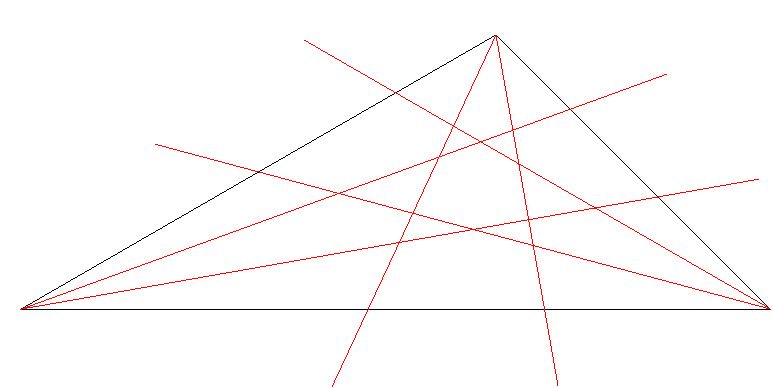
\includegraphics{./Morley_setup.pdf}%
\end{picture}%
\setlength{\unitlength}{3947sp}%
%
\begingroup\makeatletter\ifx\SetFigFont\undefined%
\gdef\SetFigFont#1#2#3#4#5{%
  \reset@font\fontsize{#1}{#2pt}%
  \fontfamily{#3}\fontseries{#4}\fontshape{#5}%
  \selectfont}%
\fi\endgroup%
\begin{picture}(6177,3093)(1036,-4420)
\put(7126,-4036){\makebox(0,0)[lb]{\smash{{\SetFigFont{12}{14.4}{\familydefault}{\mddefault}{\updefault}{\color[rgb]{0,0,0}$B$}%
}}}}
\put(1051,-4036){\makebox(0,0)[lb]{\smash{{\SetFigFont{12}{14.4}{\familydefault}{\mddefault}{\updefault}{\color[rgb]{0,0,0}$A$}%
}}}}
\put(4951,-1486){\makebox(0,0)[lb]{\smash{{\SetFigFont{12}{14.4}{\familydefault}{\mddefault}{\updefault}{\color[rgb]{0,0,0}$C$}%
}}}}
\end{picture}%

\end{center}
\caption[The setup for Morley's Miracle.]{The setup for Morley's %
Miracle -- start with an arbitrary triangle and trisect each of %
its angles.}
\label{fig:morley_setup}
\end{figure}
 
The six angle trisectors that we've just drawn intersect one another
in quite a few points.

\begin{exer}
You could literally count the number of intersection points between the
angle trisectors on the diagram, but you should also be able to count them
(perhaps we should say ``double-count them'') combinatorially.  Give it 
a try!
\end{exer}

Among the points of intersection of the angle trisectors there are three
that we will single out -- the intersections of adjacent trisectors.
In Figure~\ref{fig:morley_1st_triangle} the intersection of adjacent trisectors
are indicated, additionally, we have connected them together to form a 
small triangle in the center of our original triangle.

\clearpage

\begin{figure}[!hbtp] 
\begin{center}
\begin{picture}(0,0)%
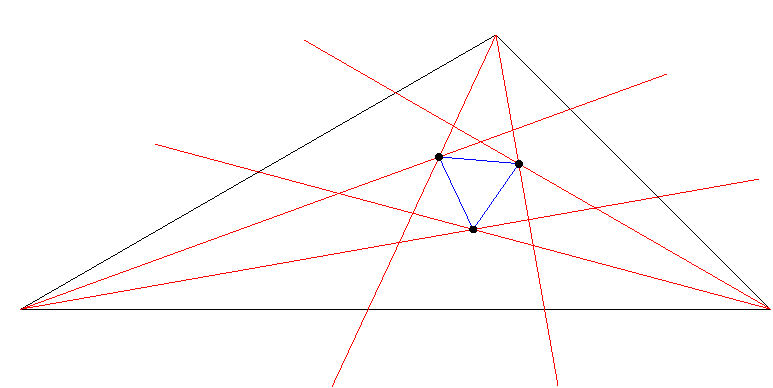
\includegraphics{figures/Morley_1st_triangle.pdf}%
\end{picture}%
\setlength{\unitlength}{3947sp}%
%
\begingroup\makeatletter\ifx\SetFigFont\undefined%
\gdef\SetFigFont#1#2#3#4#5{%
  \reset@font\fontsize{#1}{#2pt}%
  \fontfamily{#3}\fontseries{#4}\fontshape{#5}%
  \selectfont}%
\fi\endgroup%
\begin{picture}(6177,3093)(1036,-4420)
\put(1051,-4036){\makebox(0,0)[lb]{\smash{{\SetFigFont{12}{14.4}{\familydefault}{\mddefault}{\updefault}{\color[rgb]{0,0,0}$A$}%
}}}}
\put(7126,-4036){\makebox(0,0)[lb]{\smash{{\SetFigFont{12}{14.4}{\familydefault}{\mddefault}{\updefault}{\color[rgb]{0,0,0}$B$}%
}}}}
\put(4951,-1486){\makebox(0,0)[lb]{\smash{{\SetFigFont{12}{14.4}{\familydefault}{\mddefault}{\updefault}{\color[rgb]{0,0,0}$C$}%
}}}}
\end{picture}%

\end{center}
\caption[The first Morley triangle.]{A triangle is formed whose vertices %
are the intersections of the adjacent trisectors of the angles of %
${\triangle}ABC$.}
\label{fig:morley_1st_triangle}
\end{figure}
  


Are you ready for the miraculous part?  Okay, here goes!

\begin{thm}
The points of intersection of the adjacent trisectors in an arbitrary
triangle ${\triangle}ABC$ form the vertices of an equilateral triangle.
\end{thm}

In other words, that little blue triangle in 
Figure~\ref{fig:morley_1st_triangle}
that kind of \emph{looks} like it might be equilateral actually does have
all three sides equal to one another.  Furthermore, it doesn't matter what
triangle we start with, if we do the construction above we'll get
a perfect $60^\circ - 60^\circ - 60^\circ$ triangle in the middle!

 
Sources differ, but it is not clear whether Morley ever proved his 
theorem.  The first valid proof (according to R. K. Guy in~\cite{lighthouse}
was published in 1909 by M. Satyanarayana~\cite{satyana}.  There are now
\emph{many} other proofs known, for instance the cut-the-knot website
(\verb+http://www.cut-the-knot.org/+) exposits no less than nine different
proofs.  The proof by Satyanarayana used trigonometry.  The proof we'll
look at here is arguably the shortest ever produced and it is due to
\index{Conway, John}John Conway.  It is definitely a ``Book proof''!

Let us suppose that an arbitrary triangle ${\triangle}ABC$ is given.
We want to show that the triangle whose vertices are the intersections
of the adjacent trisectors is equilateral -- this triangle will be
referred to as the \index{Morley triangle}\emph{Morley triangle}.  
Let's also denote by
$A$, $B$ and $C$ the measures of the angles of ${\triangle}ABC$.  (This
is what is generally known as an ``abuse of notation'' -- we are intentionally
confounding the vertices ($A$, $B$ and $C$) of the triangle with the
measure of the angles at those vertices.)   It turns out that it is
fairly hard to reason from our knowledge of what the angles $A$, $B$ and $C$
are to deduce that the Morley triangle is equilateral.  How does the
following plan sound: suppose we construct a triangle, that definitely
\emph{does} have an equilateral Morley triangle, whose angles also happen
to be $A$, $B$ and $C$.  Such a triangle would be 
\index{similarity transform} 
similar\footnote{In Geometry, two objects are said to be \emph{similar} %
if one can be made to exactly coincide with the other after a series of %
rigid translations, rotations and scalings.  In other words, they have %
the same shape if you allow for differences in scale and are allowed to %
slide them around and spin them about as needed.} 
to the original
triangle ${\triangle}ABC$ -- if we follow the \index{similarity transform}
similarity transform from the
constructed triangle back to ${\triangle}ABC$ we will see that their 
Morley triangles must coincide; thus if one is equilateral so is the other!

One of the features of Conway's proof that leads to its great succinctness
and beauty is his introduction of some very nice notation.  
Since we are dealing with angle trisectors, let $a$, $b$ and $c$ be 
angles such that $3a=A$, $3b=B$ and $3c=C$.  Furthermore, let a superscript
star denote the angle that is $\pi/3$ (or $60^\circ$ if you prefer) greater
than a given angle.  So, for example, 

\[ a^\star = a + \pi/3 \]

\noindent and 

\[ a^{\star\star} = a + 2\pi/3. \]

Now, notice that the sum $a+b+c$ must be $\pi/3$.  This is an 
immediate consequence of $A+B+C=\pi$ which is true for any triangle
in the plane.  It follows that by distributing two stars amongst 
the three numbers $a$, $b$ and $c$ we will come up with three
quantities which sum to $\pi$.  In other words, there are 
Euclidean triangles having the following 
triples as their vertex angles:

\begin{center}
\begin{tabular}{cc}
\rule{0pt}{18pt} $(a, b, c^{\star\star})$ \rule{18pt}{0pt} & $(a, b^\star, c^\star)$ \\
\rule{0pt}{18pt} $(a, b^{\star\star}, c)$ \rule{18pt}{0pt} & $(a^\star, b^\star, c)$ \\
\rule{0pt}{18pt} $(a^{\star\star}, b, c)$ \rule{18pt}{0pt} & $(a^\star, b, c^\star)$ \\
\end{tabular}
\end{center}

\begin{exer}
What would a triangle whose vertex angles are $(0^\star, 0^\star, 0^\star)$
be?
\end{exer}

In a nutshell, Conway's proof consists of starting with an equilateral
triangle of unit side length, adding appropriately scaled versions of the 
six triangles above and ending up with a figure (having an equilateral 
Morley triangle) similar to  ${\triangle}ABC$.  The generic picture is
given in Figure~\ref{fig:morley_conway_puzzle}.  Before we can really
count this argument as a proof, we need to say a bit more about what
the phrase ``appropriately scaled'' means.  In order to appropriately
scale the triangles (the small acute ones) that appear green in Figure~\ref{fig:morley_conway_puzzle}
we have a relatively easy job -- just scale them so that the side
opposite the trisected angle has length one; that way they will join
perfectly with the central equilateral triangle.  
 
\begin{figure}[!hbtp] 
\begin{center}
\begin{picture}(0,0)%
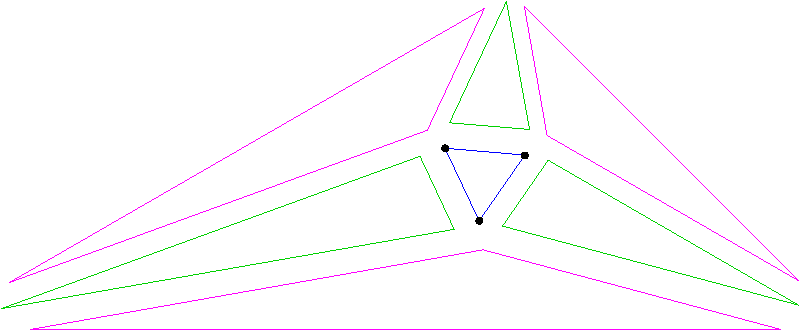
\includegraphics{figures/Morley_Conway_puzzle.pdf}%
\end{picture}%
\setlength{\unitlength}{3947sp}%
%
\begingroup\makeatletter\ifx\SetFigFont\undefined%
\gdef\SetFigFont#1#2#3#4#5{%
  \reset@font\fontsize{#1}{#2pt}%
  \fontfamily{#3}\fontseries{#4}\fontshape{#5}%
  \selectfont}%
\fi\endgroup%
\begin{picture}(6402,2682)(988,-4065)
\put(2041,-3996){\makebox(0,0)[lb]{\smash{{\SetFigFont{12}{14.4}{\familydefault}{\mddefault}{\updefault}{\color[rgb]{0,0,0}$a$}%
}}}}
\put(1771,-3676){\makebox(0,0)[lb]{\smash{{\SetFigFont{12}{14.4}{\familydefault}{\mddefault}{\updefault}{\color[rgb]{0,0,0}$a$}%
}}}}
\put(1801,-3326){\makebox(0,0)[lb]{\smash{{\SetFigFont{12}{14.4}{\familydefault}{\mddefault}{\updefault}{\color[rgb]{0,0,0}$a$}%
}}}}
\put(4791,-3566){\makebox(0,0)[lb]{\smash{{\SetFigFont{12}{14.4}{\familydefault}{\mddefault}{\updefault}{\color[rgb]{0,0,0}$c^{\star\star}$}%
}}}}
\put(4187,-2833){\makebox(0,0)[lb]{\smash{{\SetFigFont{12}{14.4}{\familydefault}{\mddefault}{\updefault}{\color[rgb]{0,0,0}$c^{\star}$}%
}}}}
\put(4321,-3206){\makebox(0,0)[lb]{\smash{{\SetFigFont{12}{14.4}{\familydefault}{\mddefault}{\updefault}{\color[rgb]{0,0,0}$b^{\star}$}%
}}}}
\put(5101,-3176){\makebox(0,0)[lb]{\smash{{\SetFigFont{12}{14.4}{\familydefault}{\mddefault}{\updefault}{\color[rgb]{0,0,0}$a^{\star}$}%
}}}}
\put(5317,-2868){\makebox(0,0)[lb]{\smash{{\SetFigFont{12}{14.4}{\familydefault}{\mddefault}{\updefault}{\color[rgb]{0,0,0}$c^{\star}$}%
}}}}
\put(4611,-1706){\makebox(0,0)[lb]{\smash{{\SetFigFont{12}{14.4}{\familydefault}{\mddefault}{\updefault}{\color[rgb]{0,0,0}$c$}%
}}}}
\put(4931,-1776){\makebox(0,0)[lb]{\smash{{\SetFigFont{12}{14.4}{\familydefault}{\mddefault}{\updefault}{\color[rgb]{0,0,0}$c$}%
}}}}
\put(5271,-1736){\makebox(0,0)[lb]{\smash{{\SetFigFont{12}{14.4}{\familydefault}{\mddefault}{\updefault}{\color[rgb]{0,0,0}$c$}%
}}}}
\put(5431,-2446){\makebox(0,0)[lb]{\smash{{\SetFigFont{12}{14.4}{\familydefault}{\mddefault}{\updefault}{\color[rgb]{0,0,0}$a^{\star\star}$}%
}}}}
\put(5013,-2380){\makebox(0,0)[lb]{\smash{{\SetFigFont{12}{14.4}{\familydefault}{\mddefault}{\updefault}{\color[rgb]{0,0,0}$b^{\star}$}%
}}}}
\put(4151,-2396){\makebox(0,0)[lb]{\smash{{\SetFigFont{12}{14.4}{\familydefault}{\mddefault}{\updefault}{\color[rgb]{0,0,0}$b^{\star\star}$}%
}}}}
\put(4681,-2346){\makebox(0,0)[lb]{\smash{{\SetFigFont{12}{14.4}{\familydefault}{\mddefault}{\updefault}{\color[rgb]{0,0,0}$a^{\star}$}%
}}}}
\put(6796,-3266){\makebox(0,0)[lb]{\smash{{\SetFigFont{12}{14.4}{\familydefault}{\mddefault}{\updefault}{\color[rgb]{0,0,0}$b$}%
}}}}
\put(6676,-3596){\makebox(0,0)[lb]{\smash{{\SetFigFont{12}{14.4}{\familydefault}{\mddefault}{\updefault}{\color[rgb]{0,0,0}$b$}%
}}}}
\put(6596,-3976){\makebox(0,0)[lb]{\smash{{\SetFigFont{12}{14.4}{\familydefault}{\mddefault}{\updefault}{\color[rgb]{0,0,0}$b$}%
}}}}
\end{picture}%

\end{center}
\caption[Conway's puzzle proof.]{Conway's proof involves putting 
these pieces together to obtain a triangle (with an equilateral
Morley triangle) that is similar to  %
${\triangle}ABC$.}
\label{fig:morley_conway_puzzle}
\end{figure}
  
The triangles (these are the larger obtuse ones) that appear purple in \ref{fig:morley_conway_puzzle} are 
a bit more puzzling.  Ostensibly, we have two different jobs to accomplish --
we must scale them so that both of the edges that they will share
with green triangles have the correct lengths.  How do we know
that this won't require two different scaling factors?  Conway also
developed an elegant argument that handles this question as well.
Consider the purple triangle at the bottom of the 
diagram in Figure~\ref{fig:morley_conway_puzzle} -- it has vertex
angles $(a,b,c^{\star\star})$.  It is possible to construct triangles
similar (via reflections) to the adjacent green triangles 
$(a, b^\star, c^\star)$ and $(a^\star, b, c^\star)$ \emph{inside} of
triangle $(a,b,c^{\star\star})$.  To do this just construct two lines that
go through the top vertex (where the angle $c^{\star\star}$ is) that cut
the opposite edge at the angle $c^\star$ in the two possible senses -- 
these two lines
will coincide if it should happen that $c^\star$ is precisely $\pi/2$
but generally there will be two and it is evident that the two line
segments formed have the same length.  We scale the purple triangle so
that this common length will be 1.  See Figure~\ref{fig:morley_conway_puzzle_scaling}.

\begin{exer}
If it should happen that $c^\star = \pi/2$, what can we 
say about $C$?
\end{exer}

\begin{figure}[!hbtp] 
\begin{center}
\begin{picture}(0,0)%
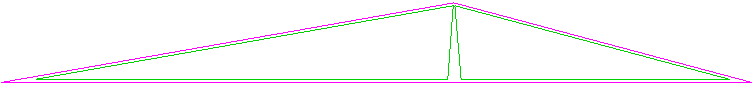
\includegraphics{./Morley_Conway_puzzle_scaling.pdf}%
\end{picture}%
\setlength{\unitlength}{3947sp}%
%
\begingroup\makeatletter\ifx\SetFigFont\undefined%
\gdef\SetFigFont#1#2#3#4#5{%
  \reset@font\fontsize{#1}{#2pt}%
  \fontfamily{#3}\fontseries{#4}\fontshape{#5}%
  \selectfont}%
\fi\endgroup%
\begin{picture}(6022,694)(1221,-4065)
\put(2041,-3996){\makebox(0,0)[lb]{\smash{{\SetFigFont{12}{14.4}{\familydefault}{\mddefault}{\updefault}{\color[rgb]{0,0,0}$a$}%
}}}}
\put(6438,-3978){\makebox(0,0)[lb]{\smash{{\SetFigFont{12}{14.4}{\familydefault}{\mddefault}{\updefault}{\color[rgb]{0,0,0}$b$}%
}}}}
\put(4634,-3603){\makebox(0,0)[lb]{\smash{{\SetFigFont{12}{14.4}{\familydefault}{\mddefault}{\updefault}{\color[rgb]{0,0,0}$b^{\star}$}%
}}}}
\put(4605,-3971){\makebox(0,0)[lb]{\smash{{\SetFigFont{12}{14.4}{\familydefault}{\mddefault}{\updefault}{\color[rgb]{0,0,0}$c^{\star}$}%
}}}}
\put(4926,-3977){\makebox(0,0)[lb]{\smash{{\SetFigFont{12}{14.4}{\familydefault}{\mddefault}{\updefault}{\color[rgb]{0,0,0}$c^{\star}$}%
}}}}
\put(4894,-3609){\makebox(0,0)[lb]{\smash{{\SetFigFont{12}{14.4}{\familydefault}{\mddefault}{\updefault}{\color[rgb]{0,0,0}$a^{\star}$}%
}}}}
\end{picture}%

\end{center}
\caption[Scaling in Conway's puzzle proof.]{The scaling factor for
the obtuse triangles in Conway's puzzle proof is determined so that 
the segments constructed in there midsts have unit length.}
\label{fig:morley_conway_puzzle_scaling}
\end{figure}
 
Of course the other two obtuse triangles can be handled in a similar way.

\clearpage

\noindent{\large \bf Exercises --- \thesection\ }

\begin{enumerate}
\item What value should we get if we sum all of the
angles that appear around one of the interior vertices in the 
finished diagram?  Verify that all three have the correct sum.

\begin{center}
\begin{picture}(0,0)%
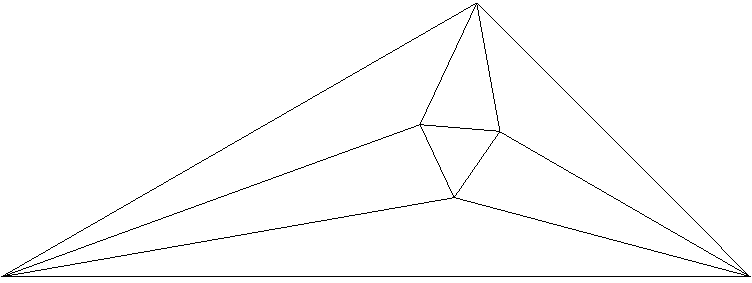
\includegraphics{figures/Morley_finished.pdf}%
\end{picture}%
\setlength{\unitlength}{3947sp}%
%
\begingroup\makeatletter\ifx\SetFigFont\undefined%
\gdef\SetFigFont#1#2#3#4#5{%
  \reset@font\fontsize{#1}{#2pt}%
  \fontfamily{#3}\fontseries{#4}\fontshape{#5}%
  \selectfont}%
\fi\endgroup%
\begin{picture}(6013,2252)(1191,-3877)
\put(1877,-3530){\makebox(0,0)[lb]{\smash{{\SetFigFont{12}{14.4}{\familydefault}{\mddefault}{\updefault}{\color[rgb]{0,0,0}$a$}%
}}}}
\put(2009,-3808){\makebox(0,0)[lb]{\smash{{\SetFigFont{12}{14.4}{\familydefault}{\mddefault}{\updefault}{\color[rgb]{0,0,0}$a$}%
}}}}
\put(1942,-3654){\makebox(0,0)[lb]{\smash{{\SetFigFont{12}{14.4}{\familydefault}{\mddefault}{\updefault}{\color[rgb]{0,0,0}$a$}%
}}}}
\put(4595,-3190){\makebox(0,0)[lb]{\smash{{\SetFigFont{12}{14.4}{\familydefault}{\mddefault}{\updefault}{\color[rgb]{0,0,0}$b^{\star}$}%
}}}}
\put(4392,-2806){\makebox(0,0)[lb]{\smash{{\SetFigFont{12}{14.4}{\familydefault}{\mddefault}{\updefault}{\color[rgb]{0,0,0}$c^{\star}$}%
}}}}
\put(4253,-2611){\makebox(0,0)[lb]{\smash{{\SetFigFont{12}{14.4}{\familydefault}{\mddefault}{\updefault}{\color[rgb]{0,0,0}$b^{\star\star}$}%
}}}}
\put(4723,-1915){\makebox(0,0)[lb]{\smash{{\SetFigFont{12}{14.4}{\familydefault}{\mddefault}{\updefault}{\color[rgb]{0,0,0}$c$}%
}}}}
\put(5094,-1936){\makebox(0,0)[lb]{\smash{{\SetFigFont{12}{14.4}{\familydefault}{\mddefault}{\updefault}{\color[rgb]{0,0,0}$c$}%
}}}}
\put(4919,-1942){\makebox(0,0)[lb]{\smash{{\SetFigFont{12}{14.4}{\familydefault}{\mddefault}{\updefault}{\color[rgb]{0,0,0}$c$}%
}}}}
\put(4683,-3383){\makebox(0,0)[lb]{\smash{{\SetFigFont{12}{14.4}{\familydefault}{\mddefault}{\updefault}{\color[rgb]{0,0,0}$c^{\star\star}$}%
}}}}
\put(6478,-3804){\makebox(0,0)[lb]{\smash{{\SetFigFont{12}{14.4}{\familydefault}{\mddefault}{\updefault}{\color[rgb]{0,0,0}$b$}%
}}}}
\put(6509,-3633){\makebox(0,0)[lb]{\smash{{\SetFigFont{12}{14.4}{\familydefault}{\mddefault}{\updefault}{\color[rgb]{0,0,0}$b$}%
}}}}
\put(6570,-3475){\makebox(0,0)[lb]{\smash{{\SetFigFont{12}{14.4}{\familydefault}{\mddefault}{\updefault}{\color[rgb]{0,0,0}$b$}%
}}}}
\put(4610,-2604){\makebox(0,0)[lb]{\smash{{\SetFigFont{12}{14.4}{\familydefault}{\mddefault}{\updefault}{\color[rgb]{0,0,0}$a^{\star}$}%
}}}}
\put(4986,-2628){\makebox(0,0)[lb]{\smash{{\SetFigFont{12}{14.4}{\familydefault}{\mddefault}{\updefault}{\color[rgb]{0,0,0}$b^{\star}$}%
}}}}
\put(5221,-2672){\makebox(0,0)[lb]{\smash{{\SetFigFont{12}{14.4}{\familydefault}{\mddefault}{\updefault}{\color[rgb]{0,0,0}$a^{\star\star}$}%
}}}}
\put(5135,-2863){\makebox(0,0)[lb]{\smash{{\SetFigFont{12}{14.4}{\familydefault}{\mddefault}{\updefault}{\color[rgb]{0,0,0}$c^{\star}$}%
}}}}
\put(4902,-3203){\makebox(0,0)[lb]{\smash{{\SetFigFont{12}{14.4}{\familydefault}{\mddefault}{\updefault}{\color[rgb]{0,0,0}$a^{\star}$}%
}}}}
\end{picture}%

\end{center}

\item In this section we talked about similarity.  Two figures in 
the plane are 
similar if it is possible to turn one into the other
by a sequence of mappings: a translation, a rotation and a scaling.  

Geometric similarity is an equivalence relation.  To fix our
notation, let $T(x,y)$ represent a generic translation, $R(x,y)$ a rotation
and $S(x,y)$ a scaling -- thus a generic similarity is a function from
$\Reals^2$ to $\Reals^2$ that can be written in the form $S(R(T(x,y)))$.

Discuss the three properties of an equivalence relation (reflexivity, symmetry and transitivity) in terms of geometric similarity.

\end{enumerate}

%% Emacs customization
%% 
%% Local Variables: ***
%% TeX-master: "GIAM-hw.tex" ***
%% comment-column:0 ***
%% comment-start: "%% "  ***
%% comment-end:"***" ***
%% End: ***



\newpage

\section{Five steps into the void}
\label{sec:5_steps}

In this section we'll talk about another Book proof also due to John
Conway.  This proof serves as an introduction to a really powerful
general technique -- the idea of an invariant.  An invariant is some
sort of quantity that one can calculate that itself doesn't change as 
other things are changed.  Of course different situations have different
invariant quantities.  

The setup here is simple and relatively intuitive.  We have a bunch
of checkers on a checkerboard -- in fact we have an infinite number
of checkers, but not filling up the whole board, they completely fill
an infinite half-plane which we could take to be the set

\[ S = \{(x,y) \suchthat x \in \Integers \, \land \, y \in \Integers \, \land \, y \leq 0 \}. \]

See Figure~\ref{fig:the_army}.
 
\begin{figure}[!hbtp] 
\begin{center}
\begin{picture}(0,0)%
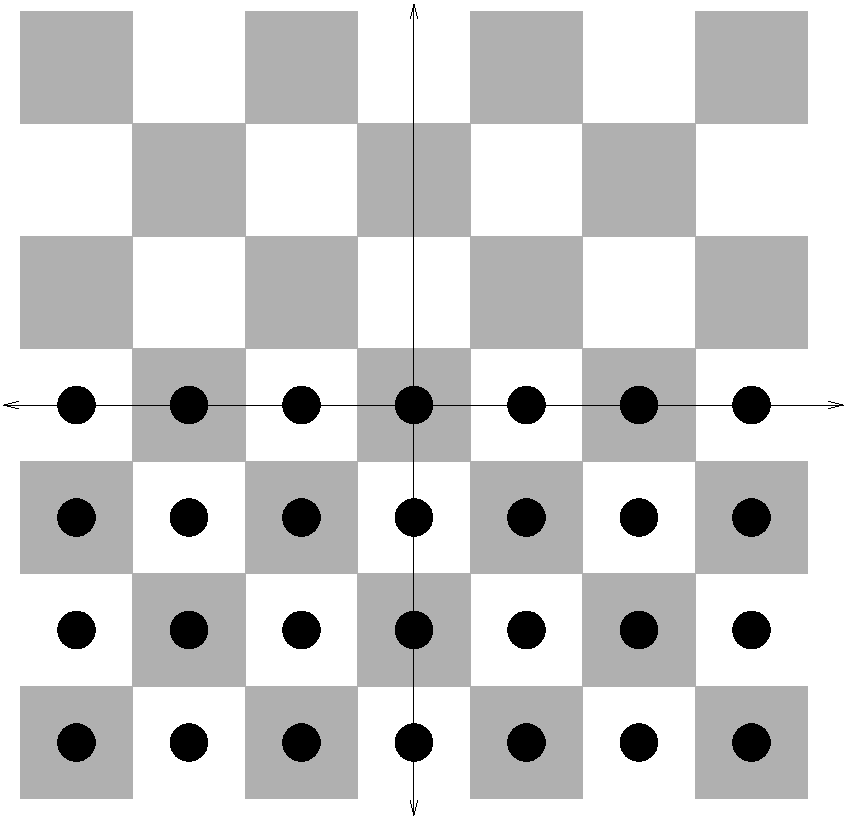
\includegraphics{./The_Army.pdf}%
\end{picture}%
\setlength{\unitlength}{3947sp}%
%
\begingroup\makeatletter\ifx\SetFigFont\undefined%
\gdef\SetFigFont#1#2#3#4#5{%
  \reset@font\fontsize{#1}{#2pt}%
  \fontfamily{#3}\fontseries{#4}\fontshape{#5}%
  \selectfont}%
\fi\endgroup%
\begin{picture}(6774,6549)(589,-8173)
\end{picture}%

\end{center}
\caption[An infinite army in the lower half-plane.]{An infinite number of
checkers occupying the integer lattice points such that $y\leq 0$.}
\label{fig:the_army}
\end{figure}
  
Think of these checkers as an army and the upper half-plane is ``enemy 
territory.''  Our goal is to move one of our soldiers into enemy territory
as far as possible.  The problem is that our ``soldiers'' move the 
way checkers do, by jumping over another man (who is then removed from 
the board).  It's clear that we can get someone into enemy territory --
just take someone in the second row and jump a guy in the first row.
It is also easy enough to see that it is possible to get a man
two steps into enemy territory -- we could bring two adjacent men
a single step into enemy territory, have one of them jump the other
and then a man from the front rank can jump over him. 

\begin{exer}
The strategy just stated uses 4 men (in the sense that they are removed
from the board -- 5 if you count the one who ends up two steps into
enemy territory as well).  Find a strategy for moving someone two
steps into enemy territory that is more efficient -- that is, involves
fewer jumps.
\end{exer}

\begin{exer}
Determine the most efficient way to get a man three steps into
enemy territory.  An actual checkers board and pieces (or some 
coins, or rocks) might come in handy.
\end{exer}

We'll count the man who ends up some number of steps above the
$x$-axis, as well as all the pieces who get jumped and removed
from the board as a measure of the efficiency of a strategy.
If you did the last exercise correctly you should have found that 
eight men are the minimum required to get 3 steps into enemy 
territory.  So far, the number of men required to get a given
distance into enemy territory seems to always be a power of 
2.

\begin{center}
\begin{tabular}{c|c}
\# of steps & \# of men \\ \hline
1 & 2 \\
2 & 4 \\
3 & 8 \\
\end{tabular}
\end{center}  

As a picture is sometimes literally worth one thousand words, we
include here 3 figures illustrating the moves necessary to put 
a scout 1, 2 and 3 steps into the void.

\begin{figure}[!hbtp] 
\begin{center}
\begin{picture}(0,0)%
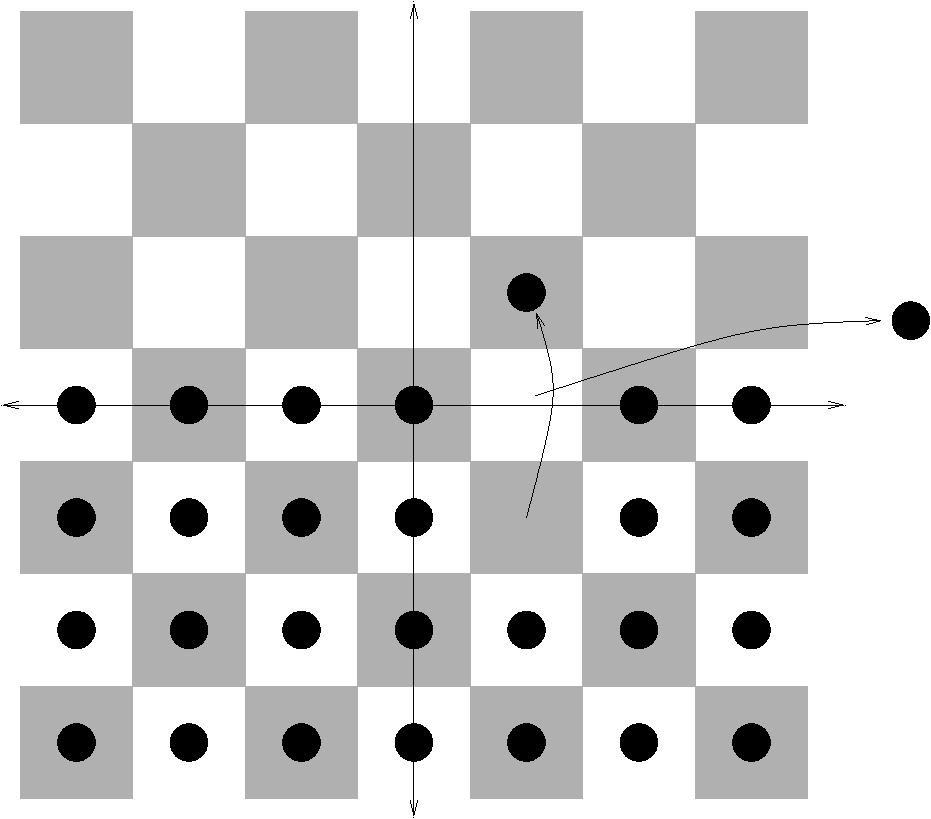
\includegraphics{figures/One_step_into_void.pdf}%
\end{picture}%
\setlength{\unitlength}{3947sp}%
%
\begingroup\makeatletter\ifx\SetFigFont\undefined%
\gdef\SetFigFont#1#2#3#4#5{%
  \reset@font\fontsize{#1}{#2pt}%
  \fontfamily{#3}\fontseries{#4}\fontshape{#5}%
  \selectfont}%
\fi\endgroup%
\begin{picture}(7445,6549)(589,-8173)
\end{picture}%

\end{center}
\caption[Moving one step into the void is trivial.]{One man is sacrificed in 
order to move a scout one step into enemy territory.}
\label{fig:one_step}
\end{figure}

\begin{figure}[!hbtp] 
\begin{center}
\begin{picture}(0,0)%
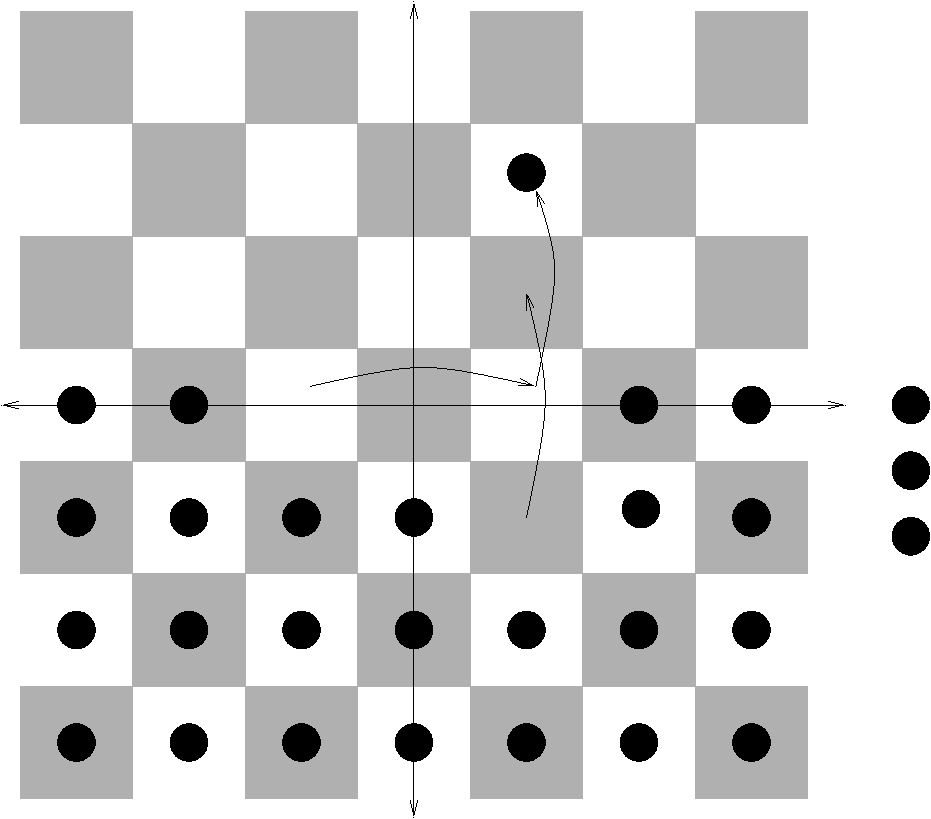
\includegraphics{./Two_steps_into_void.pdf}%
\end{picture}%
\setlength{\unitlength}{3947sp}%
%
\begingroup\makeatletter\ifx\SetFigFont\undefined%
\gdef\SetFigFont#1#2#3#4#5{%
  \reset@font\fontsize{#1}{#2pt}%
  \fontfamily{#3}\fontseries{#4}\fontshape{#5}%
  \selectfont}%
\fi\endgroup%
\begin{picture}(7445,6549)(589,-8173)
\put(5026,-4711){\makebox(0,0)[lb]{\smash{{\SetFigFont{12}{14.4}{\familydefault}{\mddefault}{\updefault}{\color[rgb]{0,0,0}1}%
}}}}
\put(4126,-4486){\makebox(0,0)[lb]{\smash{{\SetFigFont{12}{14.4}{\familydefault}{\mddefault}{\updefault}{\color[rgb]{0,0,0}2}%
}}}}
\put(5101,-3886){\makebox(0,0)[lb]{\smash{{\SetFigFont{12}{14.4}{\familydefault}{\mddefault}{\updefault}{\color[rgb]{0,0,0}3}%
}}}}
\end{picture}%

\end{center}
\caption[Moving two steps into the void is more difficult.]{Three man are sacrificed in 
order to move a scout two steps into enemy territory.}
\label{fig:two_steps}
\end{figure}

In order to show that 8 men are sufficient to get a scout 3 steps into
enemy territory, we show that it is possible to reproduce the configuration
that can place a man two steps in -- shifted up by one unit.

\begin{figure}[!hbtp] 
%\hspace{-.2in}\begin{center}
\hspace{-.2in}\begin{picture}(0,0)%
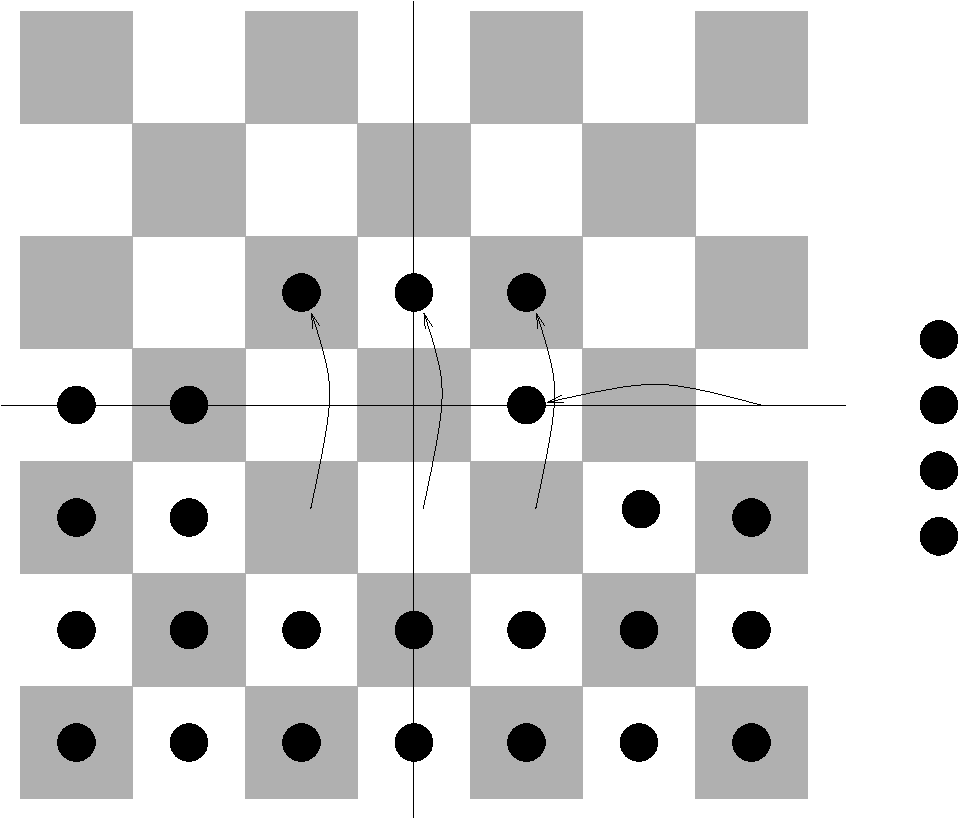
\includegraphics{./Three_steps_into_void.pdf}%
\end{picture}%
\setlength{\unitlength}{3947sp}%
%
\begingroup\makeatletter\ifx\SetFigFont\undefined%
\gdef\SetFigFont#1#2#3#4#5{%
  \reset@font\fontsize{#1}{#2pt}%
  \fontfamily{#3}\fontseries{#4}\fontshape{#5}%
  \selectfont}%
\fi\endgroup%
\begin{picture}(7670,6549)(589,-8173)
\put(3301,-4711){\makebox(0,0)[lb]{\smash{{\SetFigFont{12}{14.4}{\familydefault}{\mddefault}{\updefault}{\color[rgb]{0,0,0}1}%
}}}}
\put(4201,-4711){\makebox(0,0)[lb]{\smash{{\SetFigFont{12}{14.4}{\familydefault}{\mddefault}{\updefault}{\color[rgb]{0,0,0}2}%
}}}}
\put(5101,-4711){\makebox(0,0)[lb]{\smash{{\SetFigFont{12}{14.4}{\familydefault}{\mddefault}{\updefault}{\color[rgb]{0,0,0}3}%
}}}}
\put(5776,-4636){\makebox(0,0)[lb]{\smash{{\SetFigFont{12}{14.4}{\familydefault}{\mddefault}{\updefault}{\color[rgb]{0,0,0}4}%
}}}}
\end{picture}%

%\end{center}
\caption[Moving three steps into the void takes 8 men.]{Eight men are needed to
get a scout 3 steps into the void.}
\label{fig:three_steps}
\end{figure}

You may be surprised to learn that the pattern of 8 men which are needed to
get someone three steps into the void can be re-created -- shifted up by one
unit -- using just 12 men.  This means that we can get a man 4 steps into
enemy territory using $12 + 8 = 20$ men.  You were expecting 16 weren't you?
(I know \emph{I} was!)

\begin{exer}
Determine how to get a marker 4 steps into the void.
\end{exer}

The \emph{real} surprise is that it is simply impossible to get a man five
steps into enemy territory.  So the sequence we've been looking at actually
goes 

\[ 2, 4, 8, 20, \infty. \] 

The proof of this surprising result works by using a fairly simple, but
clever, strategy.  We assign a numerical value to a set of men that is 
dependent on their positions -- then we show that this value never increases
when we make ``checker jumping'' moves -- finally we note that the 
value assigned to a man in position $(0,5)$ is equal to the value of the
entire original set of men (that is, with \emph{all} the positions in the lower
half-plane occupied).  This is a pretty nice strategy, but how exactly are
we going to assign these numerical values?

A man's value is related to his distance from the point $(0,5)$ in what
is often called ``the taxicab metric.''   We don't use the straight-line
distance, but rather determine the number of blocks we will have to drive
in the north-south direction and in the east-west direction and add them 
together.  The value of a set of men is the sum of their individual values.
Since we need to deal with the value of the set of men that completely fills
the lower half-plane, we are going to have to have most of these values be
pretty tiny!  To put it in a more mature and dignified manner: the infinite
sum of the values of the men in our army must be convergent.

\begin{figure}[!hbtp] 
\begin{center}
\begin{picture}(0,0)%
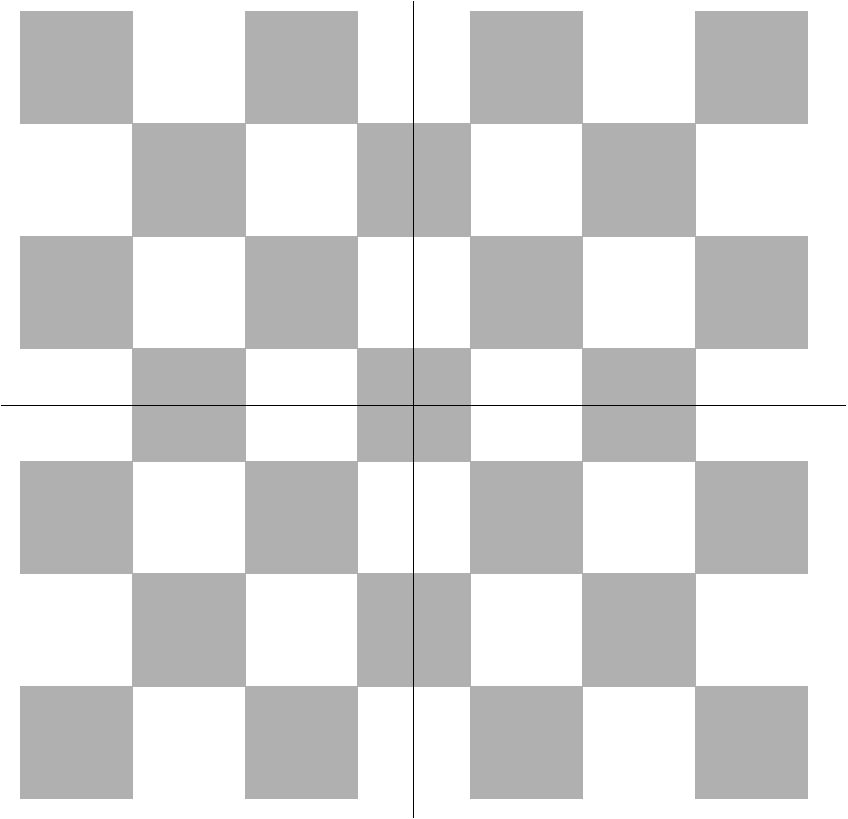
\includegraphics{figures/Taxicab_distance.pdf}%
\end{picture}%
\setlength{\unitlength}{3947sp}%
%
\begingroup\makeatletter\ifx\SetFigFont\undefined%
\gdef\SetFigFont#1#2#3#4#5{%
  \reset@font\fontsize{#1}{#2pt}%
  \fontfamily{#3}\fontseries{#4}\fontshape{#5}%
  \selectfont}%
\fi\endgroup%
\begin{picture}(6774,6549)(589,-8173)
\put(3976,-4786){\makebox(0,0)[lb]{\smash{{\SetFigFont{12}{14.4}{\familydefault}{\mddefault}{\updefault}{\color[rgb]{0,0,0}$5$}%
}}}}
\put(4801,-4786){\makebox(0,0)[lb]{\smash{{\SetFigFont{12}{14.4}{\familydefault}{\mddefault}{\updefault}{\color[rgb]{0,0,0}$6$}%
}}}}
\put(5626,-4786){\makebox(0,0)[lb]{\smash{{\SetFigFont{12}{14.4}{\familydefault}{\mddefault}{\updefault}{\color[rgb]{0,0,0}$7$}%
}}}}
\put(6601,-4786){\makebox(0,0)[lb]{\smash{{\SetFigFont{12}{14.4}{\familydefault}{\mddefault}{\updefault}{\color[rgb]{0,0,0}$8$}%
}}}}
\put(2926,-4786){\makebox(0,0)[lb]{\smash{{\SetFigFont{12}{14.4}{\familydefault}{\mddefault}{\updefault}{\color[rgb]{0,0,0}$6$}%
}}}}
\put(2101,-4786){\makebox(0,0)[lb]{\smash{{\SetFigFont{12}{14.4}{\familydefault}{\mddefault}{\updefault}{\color[rgb]{0,0,0}$7$}%
}}}}
\put(1126,-4786){\makebox(0,0)[lb]{\smash{{\SetFigFont{12}{14.4}{\familydefault}{\mddefault}{\updefault}{\color[rgb]{0,0,0}$8$}%
}}}}
\put(1126,-5761){\makebox(0,0)[lb]{\smash{{\SetFigFont{12}{14.4}{\familydefault}{\mddefault}{\updefault}{\color[rgb]{0,0,0}$9$}%
}}}}
\put(1951,-5761){\makebox(0,0)[lb]{\smash{{\SetFigFont{12}{14.4}{\familydefault}{\mddefault}{\updefault}{\color[rgb]{0,0,0}$8$}%
}}}}
\put(2926,-5761){\makebox(0,0)[lb]{\smash{{\SetFigFont{12}{14.4}{\familydefault}{\mddefault}{\updefault}{\color[rgb]{0,0,0}$7$}%
}}}}
\put(3976,-5761){\makebox(0,0)[lb]{\smash{{\SetFigFont{12}{14.4}{\familydefault}{\mddefault}{\updefault}{\color[rgb]{0,0,0}$6$}%
}}}}
\put(4726,-5761){\makebox(0,0)[lb]{\smash{{\SetFigFont{12}{14.4}{\familydefault}{\mddefault}{\updefault}{\color[rgb]{0,0,0}$7$}%
}}}}
\put(5626,-5761){\makebox(0,0)[lb]{\smash{{\SetFigFont{12}{14.4}{\familydefault}{\mddefault}{\updefault}{\color[rgb]{0,0,0}$8$}%
}}}}
\put(6526,-5761){\makebox(0,0)[lb]{\smash{{\SetFigFont{12}{14.4}{\familydefault}{\mddefault}{\updefault}{\color[rgb]{0,0,0}$9$}%
}}}}
\put(1951,-6661){\makebox(0,0)[lb]{\smash{{\SetFigFont{12}{14.4}{\familydefault}{\mddefault}{\updefault}{\color[rgb]{0,0,0}$9$}%
}}}}
\put(2926,-7561){\makebox(0,0)[lb]{\smash{{\SetFigFont{12}{14.4}{\familydefault}{\mddefault}{\updefault}{\color[rgb]{0,0,0}$9$}%
}}}}
\put(2926,-6661){\makebox(0,0)[lb]{\smash{{\SetFigFont{12}{14.4}{\familydefault}{\mddefault}{\updefault}{\color[rgb]{0,0,0}$8$}%
}}}}
\put(3976,-6661){\makebox(0,0)[lb]{\smash{{\SetFigFont{12}{14.4}{\familydefault}{\mddefault}{\updefault}{\color[rgb]{0,0,0}$7$}%
}}}}
\put(4651,-6661){\makebox(0,0)[lb]{\smash{{\SetFigFont{12}{14.4}{\familydefault}{\mddefault}{\updefault}{\color[rgb]{0,0,0}$8$}%
}}}}
\put(3901,-7561){\makebox(0,0)[lb]{\smash{{\SetFigFont{12}{14.4}{\familydefault}{\mddefault}{\updefault}{\color[rgb]{0,0,0}$8$}%
}}}}
\put(5626,-6661){\makebox(0,0)[lb]{\smash{{\SetFigFont{12}{14.4}{\familydefault}{\mddefault}{\updefault}{\color[rgb]{0,0,0}$9$}%
}}}}
\put(4651,-7561){\makebox(0,0)[lb]{\smash{{\SetFigFont{12}{14.4}{\familydefault}{\mddefault}{\updefault}{\color[rgb]{0,0,0}$9$}%
}}}}
\put(1126,-6661){\makebox(0,0)[lb]{\smash{{\SetFigFont{12}{14.4}{\familydefault}{\mddefault}{\updefault}{\color[rgb]{0,0,0}$10$}%
}}}}
\put(1051,-7561){\makebox(0,0)[lb]{\smash{{\SetFigFont{12}{14.4}{\familydefault}{\mddefault}{\updefault}{\color[rgb]{0,0,0}$11$}%
}}}}
\put(1951,-7561){\makebox(0,0)[lb]{\smash{{\SetFigFont{12}{14.4}{\familydefault}{\mddefault}{\updefault}{\color[rgb]{0,0,0}$10$}%
}}}}
\put(6526,-7561){\makebox(0,0)[lb]{\smash{{\SetFigFont{12}{14.4}{\familydefault}{\mddefault}{\updefault}{\color[rgb]{0,0,0}$11$}%
}}}}
\put(5551,-7561){\makebox(0,0)[lb]{\smash{{\SetFigFont{12}{14.4}{\familydefault}{\mddefault}{\updefault}{\color[rgb]{0,0,0}$10$}%
}}}}
\put(6526,-6661){\makebox(0,0)[lb]{\smash{{\SetFigFont{12}{14.4}{\familydefault}{\mddefault}{\updefault}{\color[rgb]{0,0,0}$10$}%
}}}}
\end{picture}%

\end{center}
\caption[The taxicab distance to $(0,5)$.]{The taxicab distance to $(0,5)$.}
\label{fig:taxicab_distance}
\end{figure}

We've previously seen geometric series which have convergent sums.  Recall 
the formula for such a sum is

\[ \sum_{k=0}^{\infty} ar^k  \quad = \quad \frac{a}{1-r}, \]

\noindent where $a$ is the initial term of the sum and $r$ is the common
ratio between terms.

Conway's big insight was to associate the powers of some number $r$ with
the positions on the board -- $r^k$ goes on the squares that are distance
$k$ from the target location.  If we have a man who is actually {\em at}
the target location, he will be worth $r^0$ or $1$.  We need to arrange for
two things to happen:  the sum of all the powers of $r$ in the initial setup
of the board must be less than or equal to 1, and checker-jumping moves should
result in the total value of a set of men going down or (at worst) staying 
the same.  These goals push us in different directions:  In order for the initial sum to be less
than 1, we would like to choose $r$ to be fairly small.  In order to have checker-jumping moves we need to choose $r$ to be (relatively) larger.  Is there a value of $r$ that does the trick?  Can we find a balance between these competing 
desires?

Think about the change in the value of our invariant as a checker jumping 
move gets made.  See Figure~\ref{fig:finding_r}.
 
\begin{figure}[!hbtp] 
\begin{center}
\begin{picture}(0,0)%
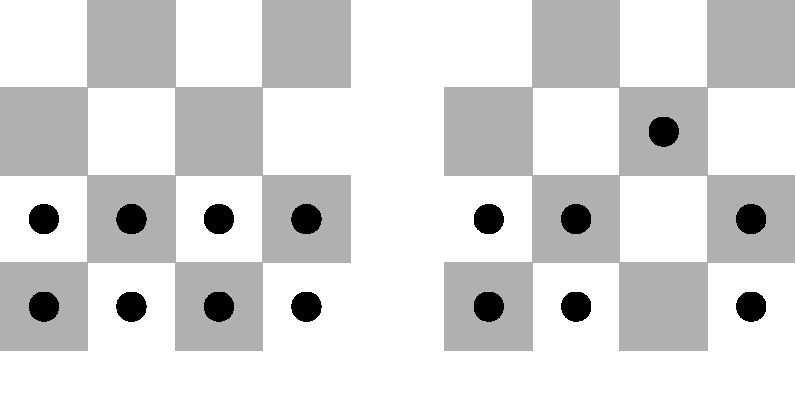
\includegraphics{figures/Void-finding_r.pdf}%
\end{picture}%
\setlength{\unitlength}{3947sp}%
%
\begingroup\makeatletter\ifx\SetFigFont\undefined%
\gdef\SetFigFont#1#2#3#4#5{%
  \reset@font\fontsize{#1}{#2pt}%
  \fontfamily{#3}\fontseries{#4}\fontshape{#5}%
  \selectfont}%
\fi\endgroup%
\begin{picture}(6360,3166)(1200,-5626)
\put(5926,-5611){\makebox(0,0)[lb]{\smash{{\SetFigFont{12}{14.4}{\rmdefault}{\mddefault}{\updefault}{\color[rgb]{0,0,0}After}%
}}}}
\put(2368,-5611){\makebox(0,0)[lb]{\smash{{\SetFigFont{12}{14.4}{\rmdefault}{\mddefault}{\updefault}{\color[rgb]{0,0,0}Before}%
}}}}
\put(3068,-5203){\makebox(0,0)[lb]{\smash{{\SetFigFont{12}{14.4}{\rmdefault}{\mddefault}{\updefault}{\color[rgb]{0,0,0}$r^{k+2}$}%
}}}}
\put(3068,-4503){\makebox(0,0)[lb]{\smash{{\SetFigFont{12}{14.4}{\rmdefault}{\mddefault}{\updefault}{\color[rgb]{0,0,0}$r^{k+1}$}%
}}}}
\put(6626,-3803){\makebox(0,0)[lb]{\smash{{\SetFigFont{12}{14.4}{\rmdefault}{\mddefault}{\updefault}{\color[rgb]{0,0,0}$r^{k}$}%
}}}}
\end{picture}%

\end{center}
\caption[Finding $r$.]{In making a checker-jump move, two men valued $r^{k+1}$ and $r^{k+2}$ are replaced by a single man valued $r^k$.}
\label{fig:finding_r}
\end{figure}
 
If we choose $r$ so that $r^{k+2} + r^{k+1} \; \leq \; r^k$ then the 
checker-jumping move will at worst leave the total sum fixed.  Note that
so long as $r<1$ a checker-jumping move that takes us away from the target 
position will certainly {\em decrease} the total sum.

As is often the case, we'll analyze the inequality by looking instead at the
corresponding equality.  What value of $r$ makes  $r^{k+2} + r^{k+1}  =  r^k$?
The answer is that $r$ must be a root of the quadratic equation $x^2+x-1$.

\begin{exer}
Do the algebra to verify the previous assertion.
\end{exer}

\begin{exer}
Find the value of $r$ that solves the above equation. 
\end{exer}

Hopefully you used the quadratic formula to solve the previous 
exercise.  You should of course have found two solutions, $-1.618033989\ldots$
and $.618033989\ldots$, these decimal approximations are actually $-\phi$ and $1/\phi$, where $\displaystyle \phi = \frac{1+\sqrt{5}}{2}$ is the famous \index{golden ratio} ``golden ratio''.   If we are hoping for the sum over all the occupied positions of $r^k$ to be convergent, we need $|r|<1$, so the negative 
solution is extraneous and so the inequality  $r^{k+2} + r^{k+1} \; \leq \; r^k$
is true in the interval $[1/\phi, 1)$.

Next we want to look at the value of this invariant when ``men'' occupy all of
the positions with $y\leq0$.  By looking at Figure~\ref{fig:taxicab_distance}
you can see that there is a single square with value $r^5$,  there are 3 squares
with value $r^6$, there are 5 squares with value $r^7$, \emph{et cetera}.
The sum, $S$, of the values of all the initially occupied positions is

\[ S \quad = \quad r^5 \cdot \sum_{k=0}^{\infty} (2k+1) r^k. \]

We have previously seen how to solve for the value of an infinite sum involving
powers of $r$.  In the expression above we have powers of $r$ but also 
multiplied by odd numbers.  Can we solve something like this?

Let's try the same trick that works for a geometric sum.  Let

\[ T \quad = \quad  \sum_{k=0}^{\infty} (2k+1) r^k \quad = \quad  1 + 3r + 5r^2 + 7r^3 + \ldots. \]

Note that 

\[ rT \quad = \quad  \sum_{k=0}^{\infty} (2k+1) r^{k+1} \quad = \quad  r + 3r^2 + 5r^3 + 7r^4 + \ldots \]

\noindent and it follows that 

\[ T - rT \quad = \quad  1 + 2 \sum_{k=1}^{\infty} r^{k} \quad = \quad 1 + 2r + 2r^2 + 2r^3 + 2r^4 + \ldots \]

A bit more algebra (and the formula for the sum of a geometric series) leads us to

\[ T = \frac{1}{1-r}\left( 1 + \frac{2r}{1-r} \right), \]

\noindent

which simplifies to 

\[ T = \frac{1+r}{(1-r)^2}. \]

Finally, recall that we are really interested in $S = r^5 \cdot T$, or

\[ S = \frac{r^5 + r^6}{(1-r)^2}. \]

It is interesting to proceed from this expression for $S$,
using the fact that $r$ satisfies $x^2 = 1 - x$, to obtain the somewhat
amazing fact that $S=1$. 

The fact that $S=1$ has an extraordinary consequence.
In order to get a single
checker to the position $(0,5)$ we would need to use \emph{everybody}!

For a set consisting of just a single
checker positioned at $(0,5)$ the value of our invariant is 1.
On the other hand, the set consisting of the entire army lined 
up on and below the $x$-axis also yields a 1.  Every checker move either
does not change the value of the invariant or reduces it.  The best 
we could possibly hope for is that there would be no need for moves 
of the sort that reduce
the invariant -- nevertheless we still could not get a man to $(0,5)$ 
in a finite number of moves.

\clearpage

\noindent{\large \bf Exercises --- \thesection\ }

\begin{enumerate}
\item Do the algebra (and show all your work!) to prove that invariant
defined in this section actually has the value 1 for the set of all the
men occupying the $x$-axis and the lower half-plane.

\wbvfill

\workbookpagebreak

\item ``Escape of the clones'' is a  nice puzzle, originally proposed by Maxim Kontsevich.  The game
is played on an infinite checkerboard restricted to the first quadrant -- that is the squares may be 
identified with points having integer coordinates $(x,y)$ with $x>0$ and $y>0$.  The ``clones'' are markers
(checkers, coins, small rocks, whatever\ldots) that can move in only one fashion -- if the squares immediately
above and to the right of a clone are empty, then it can make a ``clone move.''   The clone moves one space
up and a copy is placed in the cell one to the right.  We begin with three clones occupying cells $(1,1), (2,1)$ and $(1,2)$ -- we'll refer to those three checkerboard squares as ``the prison.''  The question is this:  can these
three clones escape the prison?

You must either demonstrate a sequence of moves that frees all three clones or provide an argument that the task is impossible.

\wbvfill

\end{enumerate}

%% Emacs customization
%% 
%% Local Variables: ***
%% TeX-master: "GIAM-hw.tex" ***
%% comment-column:0 ***
%% comment-start: "%% "  ***
%% comment-end:"***" ***
%% End: ***



\newpage

\section{Monge's circle theorem}
\label{sec:monge}

There's a nice sequence of matchstick puzzles that starts with
``Use nine non-overlapping matchsticks to form 4 triangles (all of
the same size.''  It's not that hard, and after a while most people come
up with 


\begin{center}
\begin{picture}(0,0)%
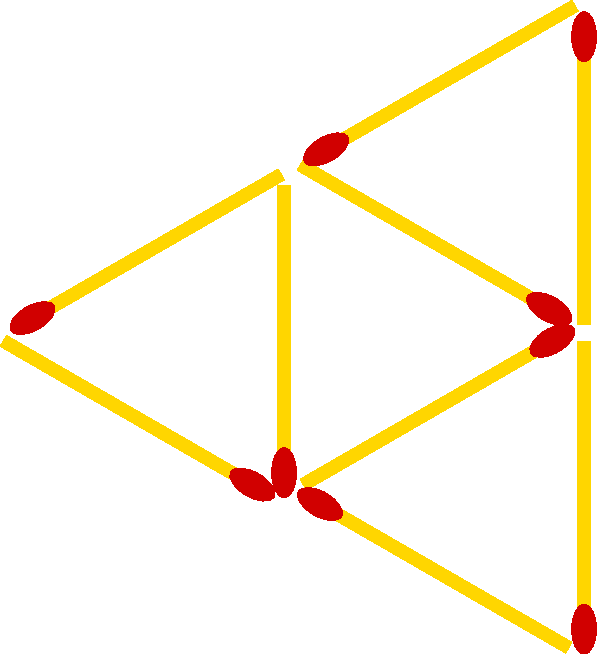
\includegraphics{figures/matchstick_puzzle.pdf}%
\end{picture}%
\setlength{\unitlength}{3947sp}%
%
\begingroup\makeatletter\ifx\SetFigFont\undefined%
\gdef\SetFigFont#1#2#3#4#5{%
  \reset@font\fontsize{#1}{#2pt}%
  \fontfamily{#3}\fontseries{#4}\fontshape{#5}%
  \selectfont}%
\fi\endgroup%
\begin{picture}(4772,5230)(1225,-4429)
\end{picture}%

\end{center}

The kicker comes when you next ask them to ``use six matches to form
4 (equal sized) triangles.''   There's a picture of the solution to
this new puzzle at the back of this section.  The answer involves 
thinking three-dimensionally, so -- with that hint -- give it a try for a
while before looking in the back.

\index{Monge's circle theorem}Monge's circle theorem has 
nothing to do with matchsticks, but it is a
\emph{sweet} example of a proof that works by moving to a higher dimension.
People often talk about ``thinking outside of the box'' when discussing
critical thinking, but the mathematical idea of moving to a higher dimension
is even more powerful.  When we have a ``box'' in 2-dimensional space which
we then regard as sitting in a 3-dimensional space we find that the box
doesn't even \emph{have} an inside or an outside anymore!  We get ``outside 
the box'' by literally erasing the notion that there \emph{is} an inside
of the box!

The setup for Monge's circle theorem consists of three random circles
drawn in the plane.  Well, to be honest they can't be entirely random --
we can't allow a circle that is entirely inside another circle.  Because,
if a circle was entirely inside another, there would be no external tangents
and Monge's circle theorem is about external tangents.

I could probably write a few hundred words to explain the concept of 
external tangents to a pair of circles, or you could just have a look at
Figure~\ref{fig:monge1}.  So, uhmm, just have a look\ldots

\begin{figure}[!hbtp] 
\begin{center}
\begin{picture}(0,0)%
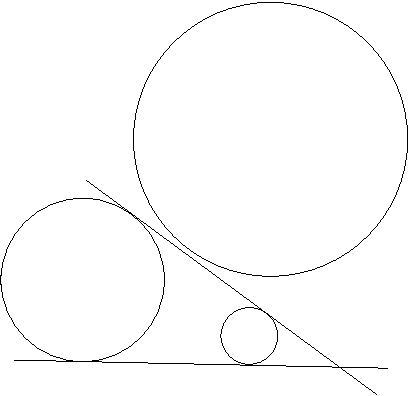
\includegraphics{./Monge_circle_setup.pdf}%
\end{picture}%
\setlength{\unitlength}{3947sp}%
%
\begingroup\makeatletter\ifx\SetFigFont\undefined%
\gdef\SetFigFont#1#2#3#4#5{%
  \reset@font\fontsize{#1}{#2pt}%
  \fontfamily{#3}\fontseries{#4}\fontshape{#5}%
  \selectfont}%
\fi\endgroup%
\begin{picture}(3270,3156)(2879,-3169)
\end{picture}%

\end{center}
\caption[Setup for Monge's circle theorem.]{The setup for Monge's circle theorem: three randomly placed circles -- we are also showing the external tangents to
one pair of circles.}
\label{fig:monge1}
\end{figure}
 
Notice how the external tangents\footnote{The reason I keep saying ``external tangents'' is that there are also \emph{internal} tangents.} to two of the circles meet in a point?  Unless the circles just happen to have exactly the same size
(And what are the odds of that?) this is going to be the case.  Each pair of external tangents are going to meet in a point.  There are three such pairs of external tangents and so they determine three points.  I suppose, since these three 
points are determined in a fairly complicated way from three randomly chosen
circles, that we would expect the three points to be pretty much random.
Monge's circle theorem says that that isn't so.

\begin{thm}[Monge's Circle Theorem] 
If three circles of different radii in the Euclidean plane are 
chosen so that no circle lies in the interior of another, the 
three pairs of external tangents to these circles meet in 
points which are collinear.
\end{thm}

In Figure~\ref{fig:monge2} we see a complete example of Monge's Circle theorem
in action.  There are three random circles.  There are three pairs of external
tangents.  The three points determined by the intersection of the pairs of 
external tangents lie on a line (shown dashed in the figure).
 
\begin{figure}[!hbtp] 
\begin{center}
\begin{picture}(0,0)%
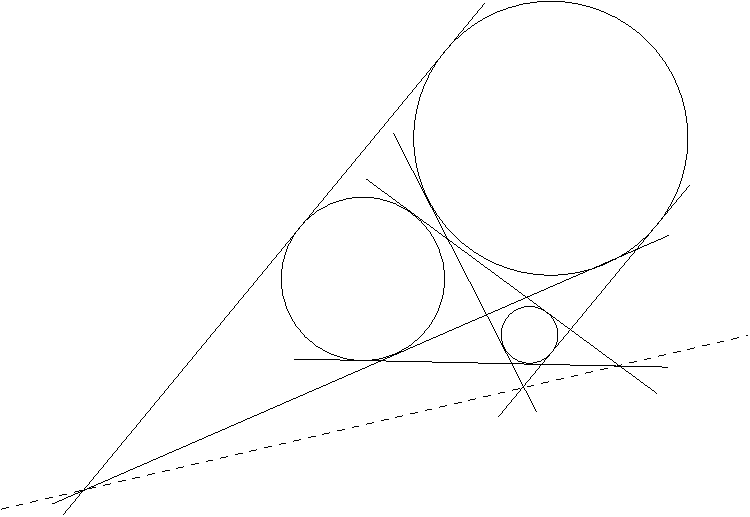
\includegraphics{figures/Monge_circle_setup_2.pdf}%
\end{picture}%
\setlength{\unitlength}{3947sp}%
%
\begingroup\makeatletter\ifx\SetFigFont\undefined%
\gdef\SetFigFont#1#2#3#4#5{%
  \reset@font\fontsize{#1}{#2pt}%
  \fontfamily{#3}\fontseries{#4}\fontshape{#5}%
  \selectfont}%
\fi\endgroup%
\begin{picture}(5992,4133)(638,-4146)
\end{picture}%

\end{center}
\caption[Example of Monge's circle theorem.]{An example of Monge's %
circle theorem.  The three pairs of external %
tangents to the circles intersect in points which are collinear.}
\label{fig:monge2}
\end{figure}
 
We won't even try to write-up a formal proof of the circle theorem.
Not that it can't be done -- it's just that you can probably get the
point better via an informal discussion.

The main idea is simply to move to 3-dimensional space.  Imagine the
original flat plane containing our three random circles as being the
plane $z=0$ in Euclidean 3-space.  Replace the three circles by three
spheres of the same radius and having the same centers -- clearly the 
intersections of these spheres with the plane $z=0$ will be our original
circles.  While pairs of circles are encompassed by two lines (the external
tangents that we've been discussing so much), when we have a pair of spheres
in 3-space, they are encompassed by a cone which lies tangent to both
spheres\footnote{As before, when the spheres happen to have identical radii %
we get a degenerate case -- the cone becomes a cylinder.}.  Notice that 
the cones that lie tangent to a pair of spheres intersect the plane
precisely in those infamous external tangents.

Well, okay, we've moved to 3-d.  We've replaced our circles with spheres
and our external tangents with tangent cones.  The points of intersection
of the external tangents are now the tips of the cones.  But, what good has this all done?
Is there any reason to believe that the tips of those cones lie in a line?

Actually, yes!  There is a plane that touches all three spheres tangentially.
Actually, there are two such planes, one that touches them all on their
upper surfaces and one that touches them all on their lower surfaces.  Oh 
damn!  There are actually \emph{lots} of planes that are tangent to all three spheres
but only one that lies above the three of them.  That plane intersects the
plane $z=0$ in a line -- nothing fancy there; any pair of non-parallel planes
will intersect in a line (and the only way the planes we are discussing
would be parallel is if all three spheres just happened to be the same size).
But that plane also lies tangent to the cones that envelope our spheres
and so that plane (as well as the plane $z=0$) contains the tips of the
cones!

\clearpage

\rule{0pt}{0pt}

\vfill

\begin{figure}[!hbtp] 
\begin{center}
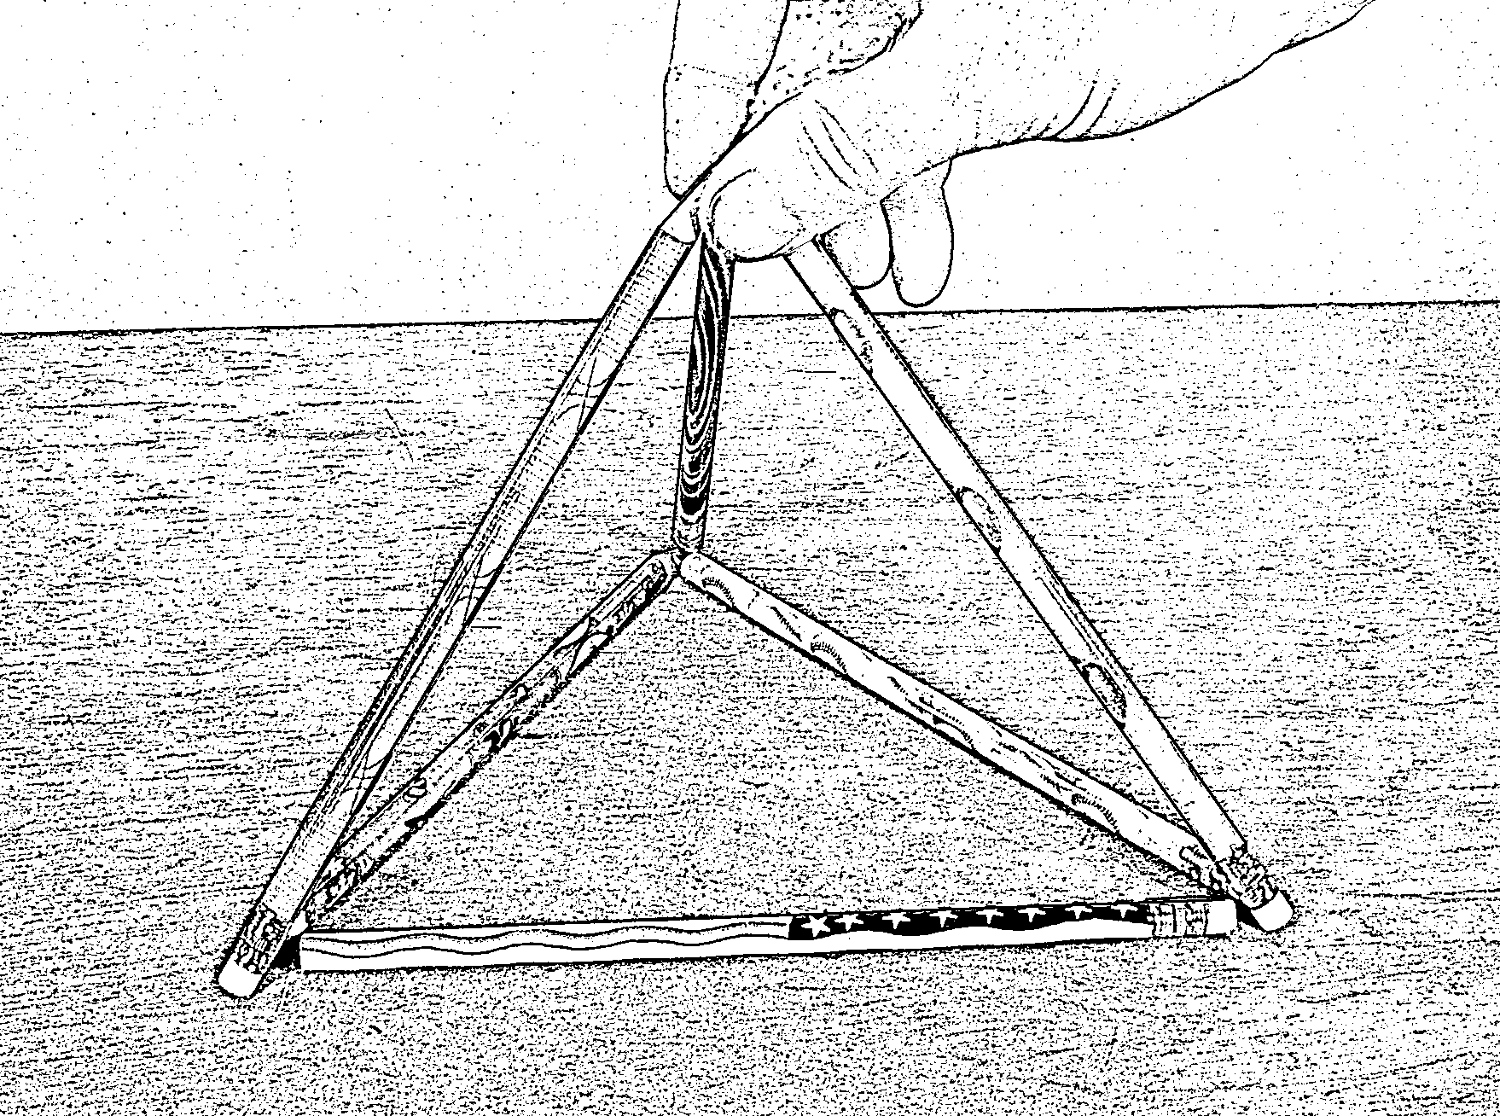
\includegraphics[scale=1]{photos/pencil_tetrahedron.jpg}
\end{center}
\caption[Four triangles bounded by 6 line segments]{Six matchstick (actually, pencils are a lot easier to hold) can be arranged three-dimensionally to create
four triangles.}
\label{fig:4triangles}
\end{figure}
 
\vfill

\rule{0pt}{0pt}

\clearpage

\noindent{\large \bf Exercises --- \thesection\ }

\begin{enumerate}
\item There is a scenario where the proof we have sketched for
Monge's circle theorem doesn't really work.  Can you envision it?
Hint: consider two relatively large spheres and one that is quite
small.
\end{enumerate}



%% Emacs customization
%% 
%% Local Variables: ***
%% TeX-master: "GIAM-hw.tex" ***
%% comment-column:0 ***
%% comment-start: "%% "  ***
%% comment-end:"***" ***
%% End: ***



%% Emacs customization
%% 
%% Local Variables: ***
%% TeX-master: "GIAM.tex" ***
%% comment-column:0 ***
%% comment-start: "%% "  ***
%% comment-end:"***" ***
%% End: ***

